%%%%%%%%%%%%%%%%%%%% author.tex %%%%%%%%%%%%%%%%%%%%%%%%%%%%%%%%%%%
%
% Conference version of the web performance optimization paper
% Adapted for Springer proceedings format (svproc)
%
%%%%%%%%%%%%%%%% Springer %%%%%%%%%%%%%%%%%%%%%%%%%%%%%%%%%%

\documentclass{svproc}

\usepackage{url}
\def\UrlFont{\rmfamily}
\usepackage{amsmath,amssymb}
\usepackage{graphicx}
\usepackage{booktabs}
\usepackage{multirow}
\usepackage{float}

\begin{document}
\mainmatter

\title{A Unified Predictive-Prescriptive-Explainable AI Pipeline for Automated Web Performance Engineering}

\titlerunning{Unified AI Pipeline for Web Performance Engineering}

\author{Shrimant A. Chavan\inst{1} \and Pratiksha R. Deshmukh\inst{1}}
%
\authorrunning{S. A. Chavan and P. R. Deshmukh}
%
\tocauthor{Shrimant A. Chavan, Pratiksha R. Deshmukh}
%
\institute{Department of Computer Engineering, COEP Technological University,
Wellesley Road, Pune 411005, Maharashtra, India\\
\email{\{chavansa24.comp, dpr.comp\}@coeptech.ac.in}}

\maketitle

\begin{abstract}
Diagnosing poor web performance is only half the battle; practitioners also need clear, trustworthy guidance on exactly what to fix. This paper introduces a unified three-phase pipeline that covers the full remediation cycle: a leak-proof predictive classifier, a direction-aware prescriptive optimizer, and a multi-method explainability layer. An XGBoost model trained on 885 real-world webpages enriched with Core Web Vitals from the Google PageSpeed Insights API achieves 90.60\% test accuracy within a scikit-learn Pipeline that prevents data leakage across cross-validation folds. The model transfers to an independent corpus of 8,000 HTTP Archive URLs at 97.54\% accuracy, establishing strong cross-dataset generalizability. A Differential Evolution engine translates predictions into domain-compliant feature prescriptions with a 100\% batch success rate. Beyond routine SHAP and LIME reporting, the explainability layer contributes a fidelity-weighted consensus ranking, quantitative stability analysis, category-stratified feature importance, and hybrid counterfactual explanations that reveal an actionability gap: timing features such as TTI and TBT appear far more frequently in counterfactuals than their SHAP importance ranks suggest. A controlled real-world experiment independently confirms the pipeline, reducing Largest Contentful Paint by 97.3\% and raising the Google PageSpeed score from 55 to 100.
\keywords{web performance optimization, predictive-prescriptive analytics, explainable AI, cross-dataset generalizability, Core Web Vitals}
\end{abstract}

% ====================================================================
%  SECTION 1 - INTRODUCTION
% ====================================================================
\section{Introduction}

Page load speed directly influences conversion rates, search-engine rankings, and user retention~\cite{kaushik2024,xin2023}. Google's introduction of Core Web Vitals as a ranking signal has elevated performance optimization from a background concern to a first-order engineering priority~\cite{mathur2024,vanriet2023}. Despite this urgency, today's tooling remains largely reactive: platforms such as Lighthouse and WebPageTest identify bottlenecks but stop short of recommending or implementing fixes.

Three research traditions address complementary aspects of this problem. Predictive approaches use machine learning to classify or forecast performance states from structural and runtime features~\cite{ghattas2025,mathur2024,sehwag2024,huang2023}. Prescriptive approaches recommend corrective actions to improve a diagnosed state~\cite{notz2024,surianarayanan2023,goscien2025,asha2025}. Explainable AI (XAI) techniques such as SHAP and LIME provide transparent reasoning behind automated decisions~\cite{salih2024,hassija2024,ortigossa2024}. Each tradition has produced valuable results independently, yet their tight integration within a single, externally validated pipeline remains rare.

Several gaps persist. Most predictive studies lack rigorous cross-validation safeguards against data leakage and formal statistical significance tests. Explainability analyses seldom go beyond a summary SHAP plot, with no stability analysis, no inter-method comparison, and no counterfactual reasoning. Small, hand-curated datasets raise legitimate concerns about generalizability to the broader web. This paper addresses all of these gaps within a single cohesive framework. The core contributions are:

\begin{enumerate}
    \item A leak-proof XGBoost pipeline confirmed by Friedman, Wilcoxon, and McNemar significance tests.
    \item A cross-dataset generalizability study on 8,000 HTTP Archive URLs achieving 97.54\% transfer accuracy.
    \item A direction-aware Differential Evolution prescriptive engine with 100\% batch success.
    \item Four novel explainability advances: fidelity-weighted consensus ranking, quantitative stability analysis, category-stratified Kruskal-Wallis testing, and hybrid counterfactual generation.
    \item A controlled real-world validation experiment that independently verifies prescriptive outputs via the external Google PageSpeed Insights API.
\end{enumerate}

% ====================================================================
%  SECTION 2 - RELATED WORK
% ====================================================================
\section{Related Work}

\textbf{Predictive modelling:} Ghattas et al.~\cite{ghattas2025} and Kaushik et al.~\cite{kaushik2024} showed that DOM complexity and micro-frontend composition can separate performance classes with standard supervised learners. Sehwag et al.~\cite{sehwag2024} applied deep learning to perceived latency through predictive prefetching, while Mathur et al.~\cite{mathur2024} quantified the link between latency and conversion rate drops. At the infrastructure layer, ensemble methods have been applied to cloud workload prediction~\cite{huang2023} and anomaly detection~\cite{xin2023}, and Daki\'{c} et al.~\cite{dakic2025} addressed Kubernetes scheduling for web workloads. None of these studies couple prediction with a systematic mechanism for acting on the diagnosed state.

\textbf{Prescriptive optimization:} Van Riet et al.~\cite{vanriet2023} documented through an industrial case study how performance engineering still depends on expert intuition and ad-hoc trial-and-error. Notz and Pibernik~\cite{notz2024} proposed mapping system states directly to optimal decisions via explainable subgradient tree boosting. Meta-heuristic methods have gained traction in adjacent domains: Asha and Ramya~\cite{asha2025} applied Predator Crow Search under non-linear constraints, and Surianarayanan et al.~\cite{surianarayanan2023} surveyed evolutionary algorithms for edge AI optimization. Hybrid heuristic-learning systems were explored by Liu et al.~\cite{liu2023} and Go\'{s}cie\'{n}~\cite{goscien2025} for resource placement tasks. Yang et al.~\cite{yang2025} combined ML-driven decision support with embedded XAI for healthcare web platforms. Despite this progress, direct application of prescriptive optimization to web performance features with direction-aware domain constraints remains limited.

\textbf{Explainability:} The deployment of opaque models in reliability-sensitive loops raises trust and transparency concerns~\cite{goyal2025,ali2023}. Surveys by Hassija et al.~\cite{hassija2024}, Mersha et al.~\cite{mersha2024}, and Ortigossa et al.~\cite{ortigossa2024} present broad XAI taxonomies, while Bennetot et al.~\cite{bennetot2024} provide a practical tutorial. Goldwasser and Hooker~\cite{goldwasser2024} studied conditions under which SHAP and LIME rankings are provably stable, and Salih et al.~\cite{salih2024} warned that collinear features can distort Shapley attribution. Hosain et al.~\cite{hosain2024} noted frequent disagreement between gradient-based and perturbation-based explanations, while Sharma et al.~\cite{zhou2024} identified a gap in systematic consensus mechanisms. Applied XAI work spans anomaly detection~\cite{alam2024}, recommender systems~\cite{benleulmi2025,rahim2025}, data augmentation~\cite{mersha2025}, and privacy-preserving frameworks~\cite{bhardwaj2025}. Ali et al.~\cite{ali2023} argued that trustworthy XAI must provide quantifiable evidence of faithfulness and stability rather than one-off visualizations. In the web performance domain, however, XAI use has been confined to single-method reporting with no stability analysis, no inter-method comparison, and no counterfactual reasoning.

% ====================================================================
%  SECTION 3 - SYSTEM ARCHITECTURE AND METHODOLOGY
% ====================================================================
\section{System Architecture and Methodology}

The framework is organized into four tightly coupled phases preceded by data enrichment and followed by real-world validation, as illustrated in Figure~\ref{fig:system_architecture}.

\subsection{Data Enrichment and Primary Dataset}

Standard performance datasets rely on static file characteristics that correlate poorly with perceived user experience~\cite{sehwag2024,huang2023}. The primary corpus of 885 unique webpages was built by merging structural records from a public repository with dynamic Core Web Vitals (LCP, TBT, CLS, FCP, TTI) retrieved from the Google PageSpeed Insights API, consistent with recent studies that treat user-centric metrics as essential for reliable performance modelling~\cite{mathur2024}. After preprocessing, 14 base features were retained and eight additional features were engineered (Table~\ref{tab:engineered_features}), yielding 22 model features in total. Performance labels (fast, medium, slow) were derived from composite thresholds across Response Time, LCP, FCP, TTI, and TBT, producing a roughly balanced class distribution: 299 fast, 271 medium, and 315 slow.

\begin{table}[htbp]
\caption{Engineered Features}\label{tab:engineered_features}
\centering
\begin{tabular}{lll}
\toprule
Feature & Formula & Rationale \\
\midrule
Size\_LoadTime\_Ratio & Page Size / Load Time & Efficiency metric \\
Total\_Time & Response Time + Load Time & Combined latency \\
Throughput\_RT\_Ratio & Throughput / Response Time & Network efficiency \\
Log\_Page\_Size & $\log_{1p}$(Page Size) & Reduce skewness \\
Log\_Throughput & $\log_{1p}$(Throughput) & Reduce skewness \\
CWV\_Composite & (LCP + FCP + TTI) / 3 & Core Web Vitals aggregate \\
TBT\_TTI\_Ratio & TBT / TTI & Main-thread blocking ratio \\
Bytes\_Per\_Request & total\_byte\_weight / num\_requests & Per-request payload \\
\bottomrule
\end{tabular}
\end{table}

\subsection{Phase 1: Leak-Proof Predictive Modelling}

Four supervised classifiers were trained: SVM (RBF kernel), Random Forest, Gradient Boosting, and XGBoost. Each was tuned with RandomizedSearchCV over 20 candidate configurations and 5-fold stratified cross-validation. All preprocessing (RobustScaler) and the classifier were wrapped inside a scikit-learn Pipeline, ensuring the scaler is fit only on training-fold data during each CV iteration and preventing the information leakage that arises when scaling is applied before splitting~\cite{xin2023,dakic2025}. The dataset was partitioned into a 70:30 stratified split (619 training, 266 test samples). Model superiority was confirmed through Friedman, Wilcoxon signed-rank, and McNemar significance tests.

\begin{figure}[htb]
    \centering
    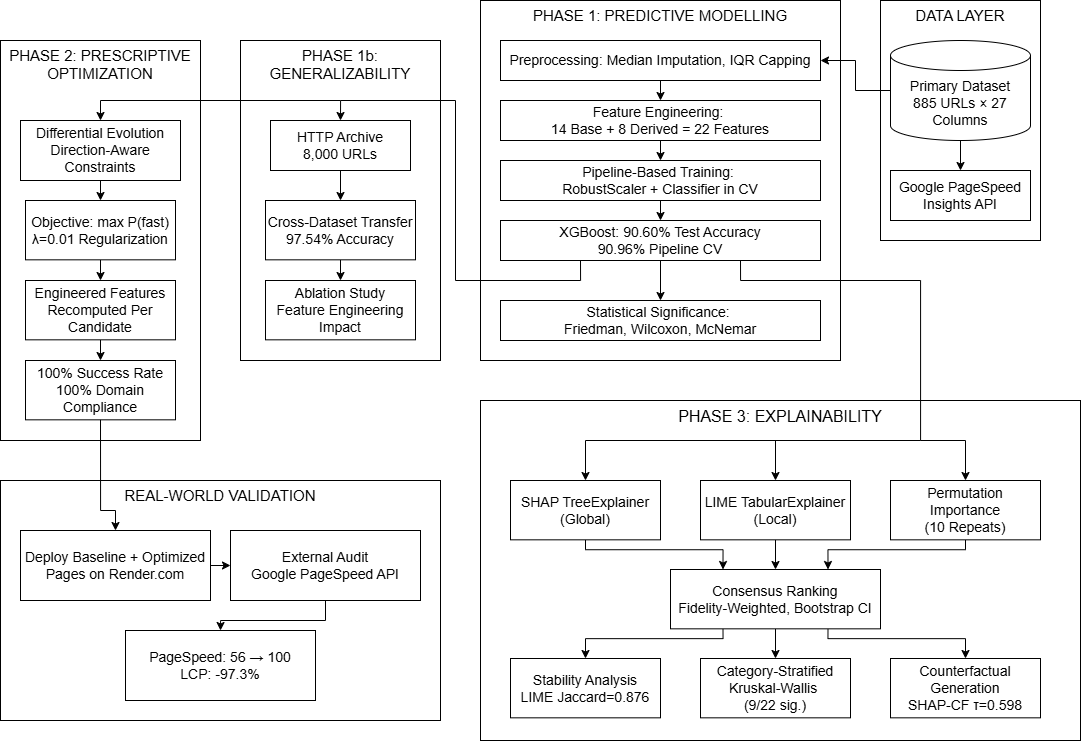
\includegraphics[width=\linewidth]{figures/NewSysArch.png}
    \caption{End-to-end system architecture. Data flows through four phases: (1)~Predictive Modelling with leak-proof Pipeline CV, (1b)~Cross-Dataset Generalizability on 8,000 HTTP Archive URLs, (2)~Prescriptive Optimization via Differential Evolution under direction-aware domain constraints, and (3)~Explainability comprising SHAP, LIME, Permutation Importance, consensus ranking, stability analysis, category-stratified testing, and counterfactual generation. A Real-World Validation loop closes the pipeline by deploying prescriptions and auditing them through the external Google PageSpeed Insights API.}
    \label{fig:system_architecture}
\end{figure}


\subsection{Phase 1b: Cross-Dataset Generalizability}

To evaluate whether the learned representations hold beyond the primary dataset, a separate study trained and evaluated models on 8,000 URLs from the HTTP Archive (December 2025 mobile crawl, Tranco top 200,000). Labels were assigned independently using Google's published thresholds for Speed Index, Load Time, and TTFB via majority vote, with no dependence on the Phase~1 model. Thirteen features common to both datasets were used for cross-dataset transfer experiments.

\subsection{Phase 2: Prescriptive Optimization Engine}

While prediction identifies the problem, Phase~2 generates a concrete solution. A Differential Evolution optimizer~\cite{asha2025} maximizes $P(\text{fast})$ for slow pages by iteratively mutating the feature vector. The objective function is:
\[
\min_{x}\left[-P(\text{fast} \mid x) + \lambda \sum_i \left(\frac{x_i - x_i^{\text{current}}}{|x_i^{\text{current}}| + \epsilon}\right)^{\!2}\right]
\]
where $\lambda = 0.01$ penalizes large deviations from the current configuration, encouraging the optimizer to find minimal, realistic changes~\cite{notz2024,surianarayanan2023}. Direction-aware constraints enforce physical plausibility: load-time metrics may only decrease, throughput may only increase, and site category is fixed. Engineered features are recomputed from base features after each candidate evaluation.

\subsection{Phase 3: Multi-Method Explainability}

The explainability layer goes beyond standard single-method reporting~\cite{hassija2024,bennetot2024}. Global SHAP via TreeExplainer~\cite{salih2024} and local LIME via LimeTabularExplainer provide attribution baselines. A fidelity-weighted consensus ranking then integrates SHAP, LIME, and Permutation Importance into a single feature ordering with bootstrap confidence intervals, with weights proportional to each method's measured fidelity~\cite{goldwasser2024}. Explanation stability is quantified by running LIME 20 times per sample (top-5 Jaccard similarity) and injecting $\pm$5\% Gaussian noise into SHAP inputs ($L_2$ drift). Category-stratified Kruskal-Wallis tests partition SHAP values by website category to detect significantly different importance patterns. Finally, hybrid counterfactual generation combines nearest-prototype seeding with growing-spheres random search under directional domain constraints to find the minimal set of changes that flips a non-fast page to fast.

\subsection{Real-World Validation}

Two contrasting web deployments were constructed: a deliberately slow baseline page (6 MB uncompressed BMP image, 500 redundant DOM nodes, synchronous Fibonacci calculation blocking the main thread) and an optimized page implementing the Phase~2 prescriptions (5 KB WebP image, deferred scripts, pruned DOM). Both were audited by the external Google PageSpeed Insights API, providing ground truth independent of the internal model and eliminating the circular validation common in prior work~\cite{vanriet2023}.

% ====================================================================
%  SECTION 4 - RESULTS AND ANALYSIS
% ====================================================================
\section{Results and Analysis}

\subsection{Predictive Model Performance}

Table~\ref{tab:model_comparison} summarizes classifier performance. XGBoost achieved the highest accuracy on both the test set (90.60\%) and in pipeline cross-validation (90.96\%). The test-to-CV gap of only $-0.36$ percentage points indicates strong generalization with no sign of overfitting. Precision (0.9063), recall (0.9060), and F1-score (0.9058) are tightly grouped, confirming balanced performance across all three classes.

\begin{table}[h]
\caption{Predictive Model Comparison (Primary Dataset, 22 Features)}\label{tab:model_comparison}
\centering
\begin{tabular}{lccc}
\toprule
Model & Test Acc. & F1-Score & CV Accuracy (Pipeline) \\
\midrule
SVM (RBF) & 36.84\% & 0.2227 & --- \\
Random Forest & 87.97\% & 0.8778 & $88.47\% \pm 1.65\%$ \\
Gradient Boosting & 89.85\% & 0.8977 & $89.60\% \pm 1.56\%$ \\
\textbf{XGBoost} & \textbf{90.60\%} & \textbf{0.9058} & $\mathbf{90.96\% \pm 1.40\%}$ \\
\bottomrule
\end{tabular}
\end{table}

SVM performed poorly at 36.84\%, as radial basis functions scale badly with the heterogeneous, mixed-type features present in web performance data~\cite{xin2023,huang2023}. The three tree-based models all exceeded 87\%, benefiting from their native capacity to handle non-linear interactions. The Friedman test confirmed that performance differences among tree-based classifiers are not due to chance ($p < 0.05$). Pairwise Wilcoxon and McNemar tests further confirmed XGBoost's superiority over all other models. The confusion matrix in Figure~\ref{fig:confusion_matrix} shows strong per-class classification with no evidence of majority-class dominated accuracy.

\begin{figure}[htb]
    \centering
    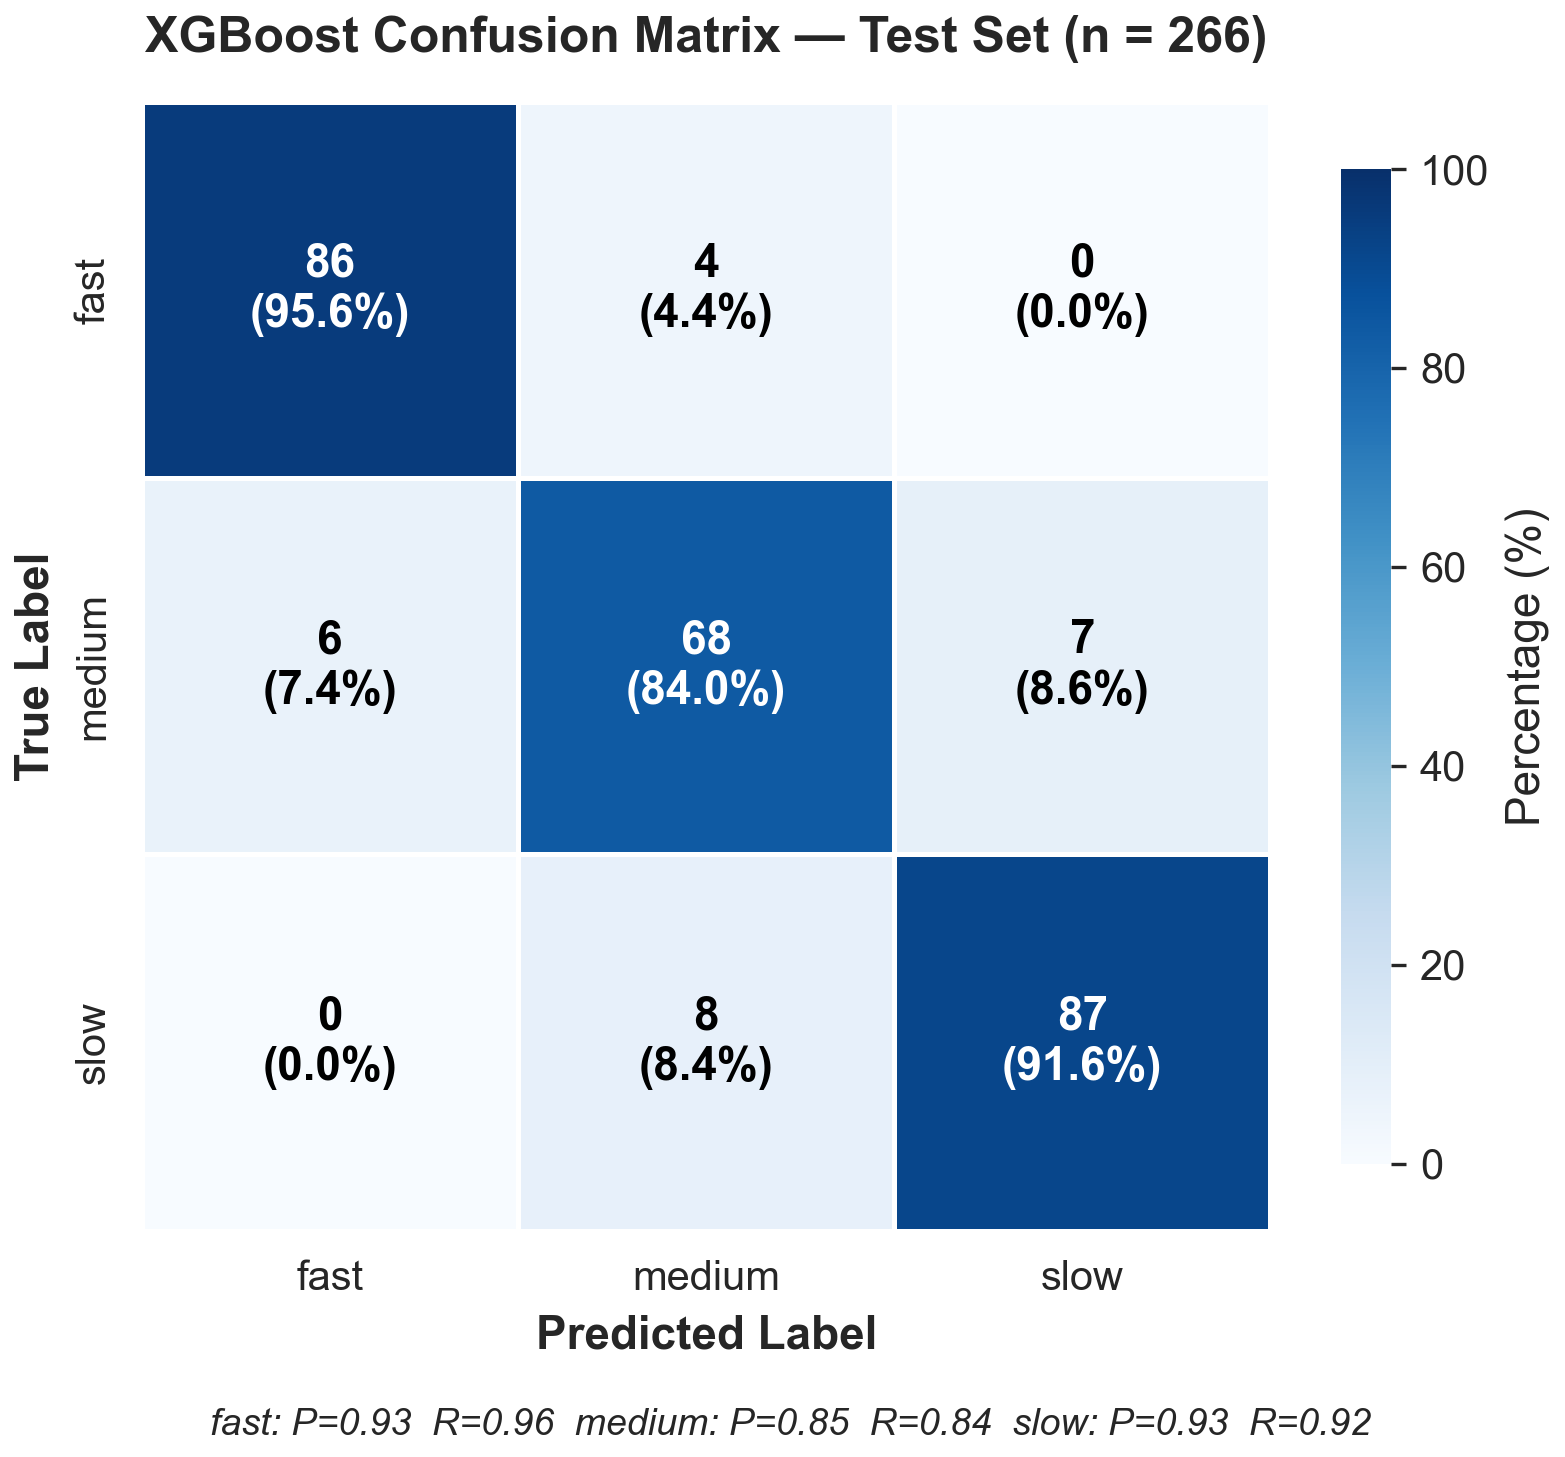
\includegraphics[width=0.7\linewidth]{figures/fig1_confusion_matrix.png}
    \caption{Confusion matrix for the XGBoost classifier on the held-out test set ($n = 266$). Each cell shows the count and row-normalised percentage. Per-class precision and recall are annotated below.}
    \label{fig:confusion_matrix}
\end{figure}

\subsection{Cross-Dataset Generalizability}

Table~\ref{tab:cross_dataset} presents transfer results. The headline figure is a model trained on 885 curated pages correctly classifying 97.54\% of 8,000 independently labelled HTTP Archive URLs, demonstrating that the learned representations capture genuine performance patterns that transfer to a much larger, independently collected corpus. The reverse transfer (88.36\%) is lower because the HA-trained model lacks exposure to the richer Core Web Vitals features that drive classification on the primary set.

\begin{table}[h]
\caption{Cross-Dataset Transfer Results}\label{tab:cross_dataset}
\centering
\begin{tabular}{lcc}
\toprule
Transfer Direction & Accuracy & F1-Score \\
\midrule
Train on Primary (885) $\rightarrow$ Test on HA (8,000) & \textbf{97.54\%} & 0.9752 \\
Train on HA (8,000) $\rightarrow$ Test on Primary (885) & 88.36\% & 0.8870 \\
\bottomrule
\end{tabular}
\end{table}

An ablation study confirmed that on the primary dataset, the full set of eight engineered features contributes a substantially larger accuracy gain (from roughly 72\% to 91\%) compared to the HA dataset, where \textit{speed\_index} alone carries 79.9\% of feature importance and the marginal gain from feature engineering is only +0.06 pp.

\subsection{Prescriptive Optimization Outcomes}

For a representative slow page, the optimizer shifted the predicted class from slow ($P(\text{fast}) = 0.0\%$) to fast ($P(\text{fast}) = 99.8\%$). The top prescriptions were: LCP reduction of 60.5\% (critical), Response Time reduction of 59.0\% (critical), TTI reduction of 32.2\% (high), FCP reduction of 28.1\% (high), and Load Time reduction of 9.2\% (medium). These align with established engineering best practices: LCP reduction calls for image compression, response time reduction points to server-side tuning, and TTI reduction requires deferring non-critical JavaScript~\cite{vanriet2023,surianarayanan2023}.

In batch evaluation across five slow pages, all five were successfully transitioned to fast with an average $P(\text{fast})$ improvement of +0.95 and 100\% domain compliance. Every one of the 12 individual recommendations was directionally correct, confirming that the optimizer navigates the 22-dimensional feature space without generating physically implausible suggestions.

\subsection{Explainability Results}

\textbf{Standard SHAP and LIME:} Global SHAP values identified Response Time (2.920), FCP (2.168), performance\_score (1.685), LCP (1.585), and Total\_Time (1.462) as the five strongest performance drivers, confirming the model has learned domain-appropriate relationships rather than artefactual correlations. Figure~\ref{fig:shap_beeswarm} presents the global importance bar chart and the beeswarm plot for the fast class. Local LIME analysis showed consistent per-instance reasoning aligned with the global SHAP rankings, and boundary cases showed nearly equal probability splits between classes, indicating genuine data ambiguity rather than model deficiency.

\begin{figure}[htb]
    \centering
    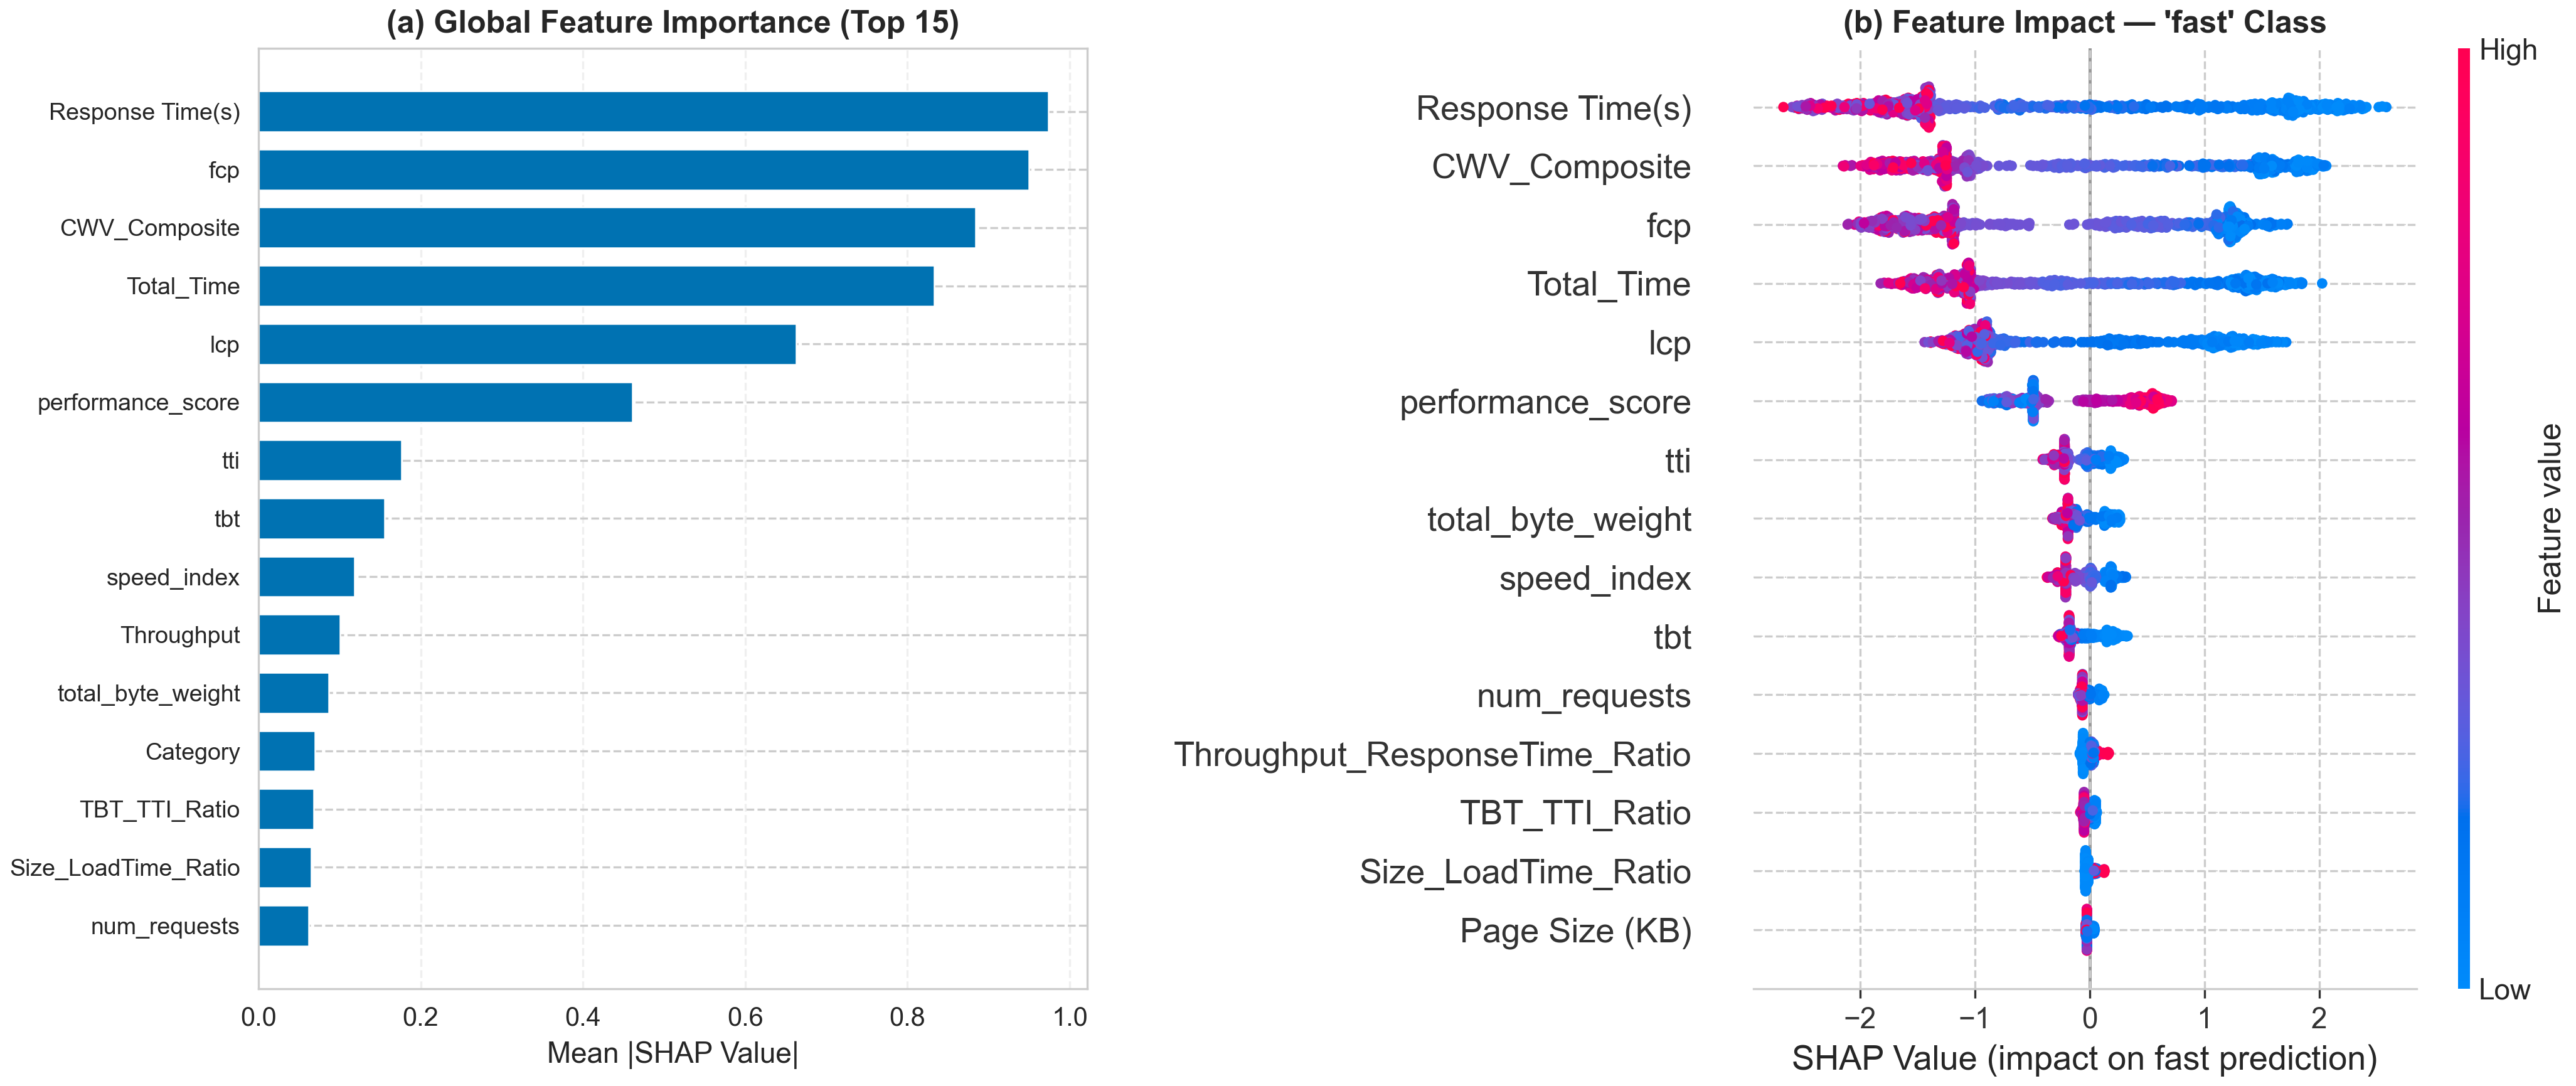
\includegraphics[width=\linewidth]{figures/fig2_shap_beeswarm.png}
    \caption{SHAP global feature importance. (a)~Mean absolute SHAP values across all classes (top 15 features). (b)~Beeswarm plot for the fast class, showing how each feature's value (colour) pushes predictions towards or away from fast.}
    \label{fig:shap_beeswarm}
\end{figure}

\textbf{Consensus Ranking (Novel Contribution 1):} Fidelity weights were: SHAP (0.438), Permutation Importance (0.438), and LIME (0.123, reflecting a mean local $R^2$ of 0.281). The top five consensus features were Response Time (0.9939), CWV\_Composite (0.8190), FCP (0.8023), Total\_Time (0.6868), and LCP (0.4918). Inter-method rank correlations (Kendall's $\tau$) ranged from 0.565 to 0.633, indicating moderate-to-strong agreement that nonetheless justifies a formal consensus over reliance on any single technique. Figure~\ref{fig:consensus_ranking} visualises the consensus scores alongside the per-method contributions.

\begin{figure}[htb]
    \centering
    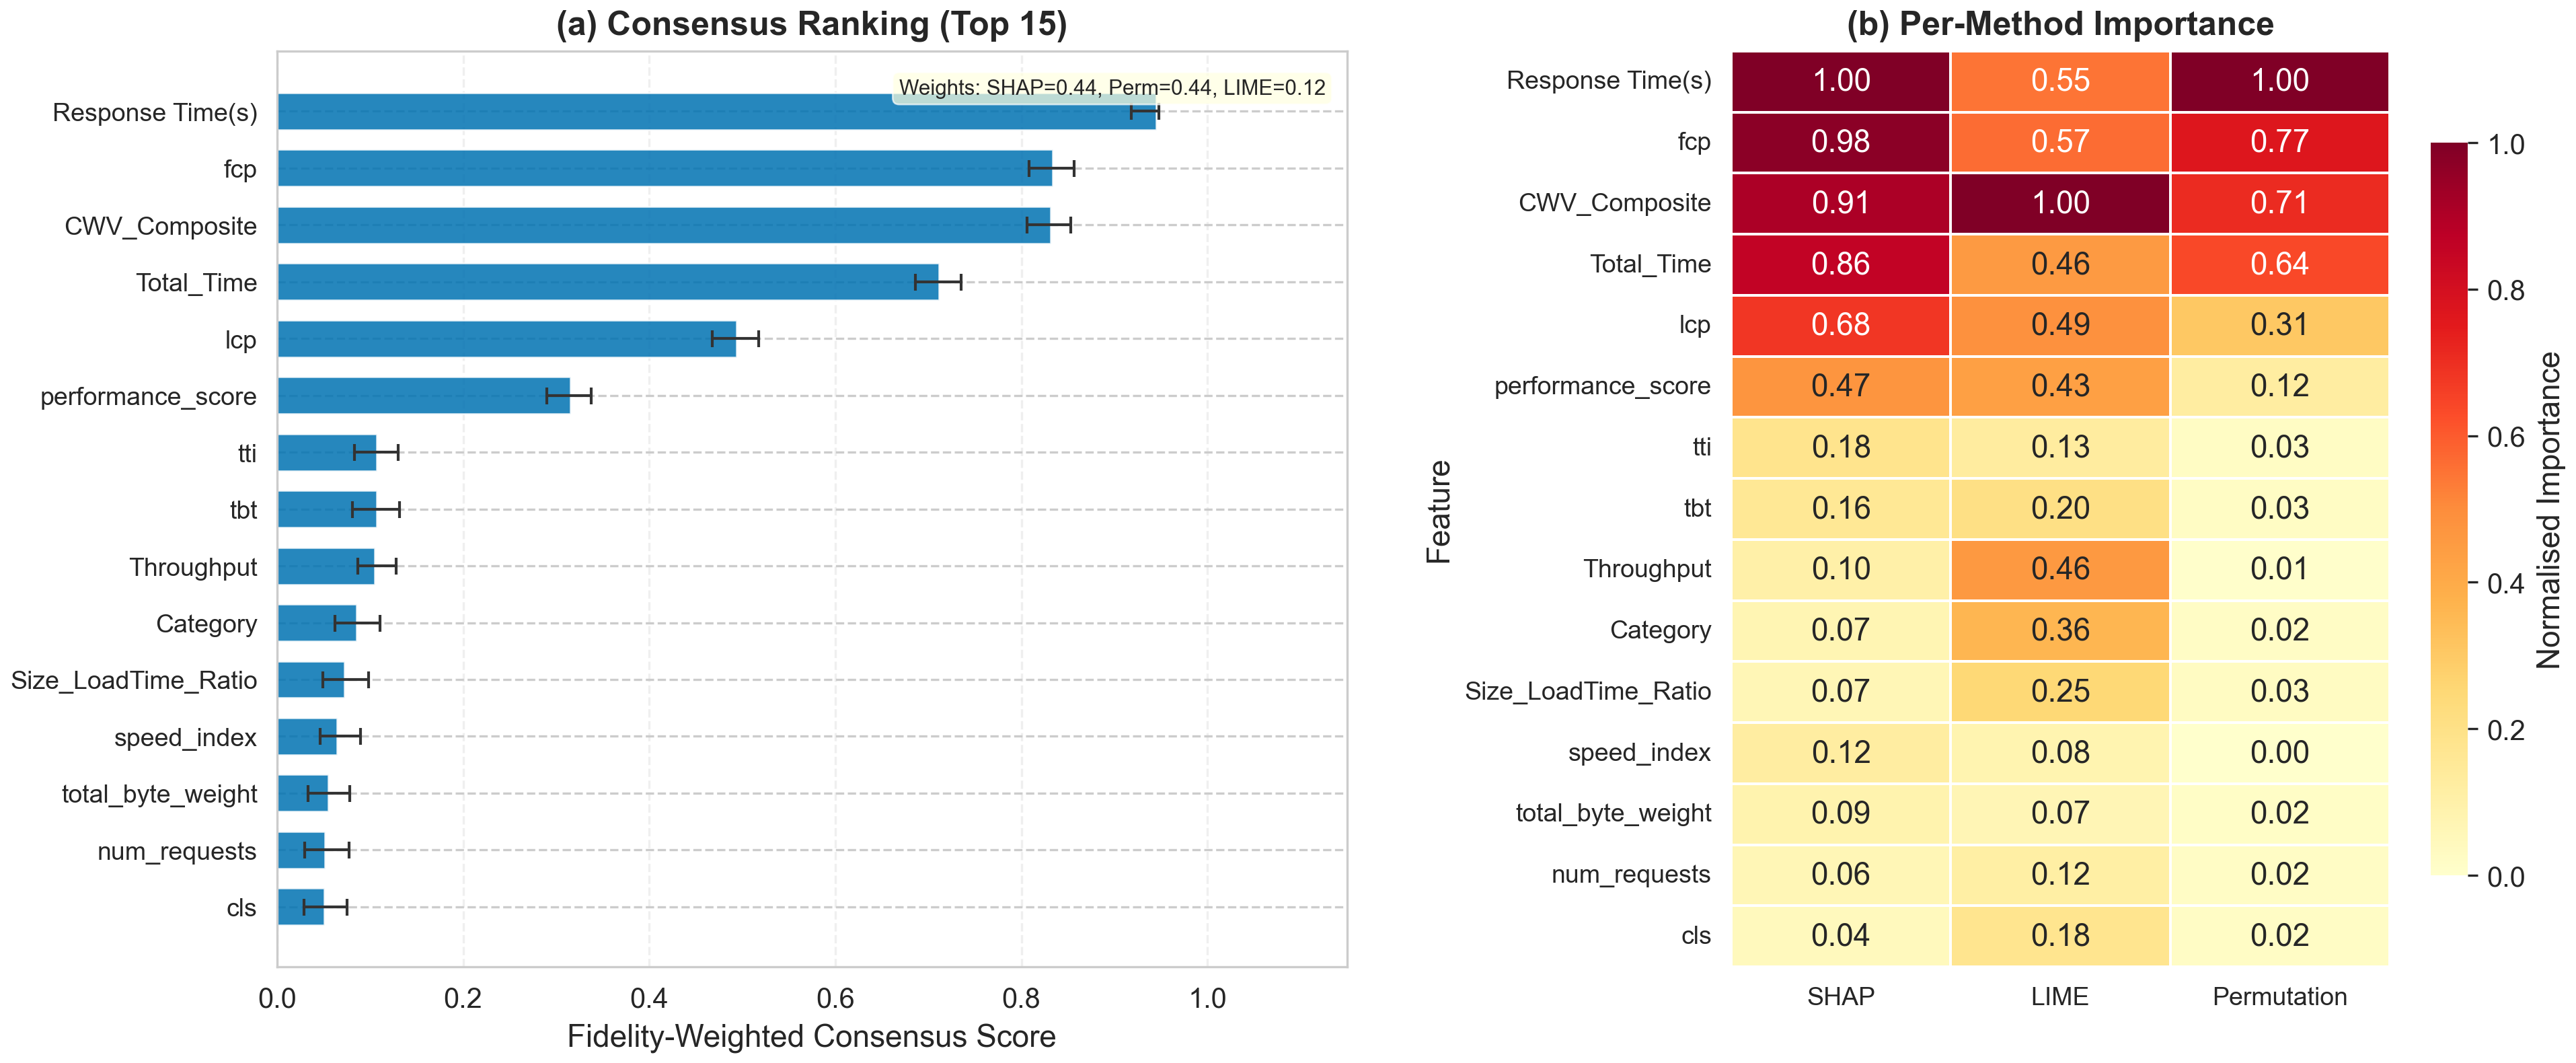
\includegraphics[width=\linewidth]{figures/fig3_consensus_ranking.png}
    \caption{Fidelity-weighted consensus ranking. (a)~Top-15 features ranked by consensus score with 95\% bootstrap confidence intervals. (b)~Per-method normalised importance heatmap (SHAP, LIME, Permutation Importance).}
    \label{fig:consensus_ranking}
\end{figure}

\textbf{Stability and Robustness (Novel Contribution 2):} Over 30 samples and 20 LIME runs each, the mean top-5 Jaccard similarity was $0.876 \pm 0.105$, exceeding the conventional 0.80 stability threshold. SHAP sensitivity under $\pm$5\% Gaussian noise produced a mean $L_2$ drift of $0.328 \pm 0.254$, indicating moderate but bounded sensitivity. Cross-method SHAP-to-LIME agreement was weakest for the medium class ($\tau = 0.342$), which is expected since the medium class sits at the decision boundary where model uncertainty is naturally highest.

\textbf{Category-Stratified Importance (Novel Contribution 3):} Kruskal-Wallis tests revealed that 9 of 22 features differed significantly across website categories ($p < 0.05$): Category, Page Size, TTI, Load Time, CLS, Size\_LoadTime\_Ratio, CWV\_Composite, num\_requests, and Throughput. While all eight categories share the same top-three drivers (Response Time, CWV\_Composite, FCP), the magnitudes differ meaningfully, supporting tailored category-specific optimization strategies rather than generic recommendations.

\textbf{Counterfactual Explanations (Novel Contribution 4):} Counterfactuals were generated for 100 non-fast samples with a 100\% success rate, changing a mean of 13.2 features per sample. Features appearing most frequently were FCP (93\%), performance\_score (91\%), CWV\_Composite (89\%), LCP (87\%), and Response Time (85\%). Timing composites TTI, TBT, and TBT\_TTI\_Ratio appeared in 75--88\% of counterfactuals despite carrying comparatively low SHAP importance scores (normalized $\leq 0.15$), revealing a meaningful actionability gap. Conversely, Category ranked 4th in global SHAP importance but appeared in almost no counterfactuals, correctly reflecting that site category is a structural property that cannot be directly optimized. The overall SHAP-to-counterfactual rank correlation was Kendall's $\tau = 0.598$, $p < 0.001$ (Spearman's $\rho = 0.772$), confirming moderate global agreement while the per-feature divergences carry significant practical implications. Figure~\ref{fig:shap_vs_cf} makes this divergence visually explicit.

\begin{figure}[htb]
    \centering
    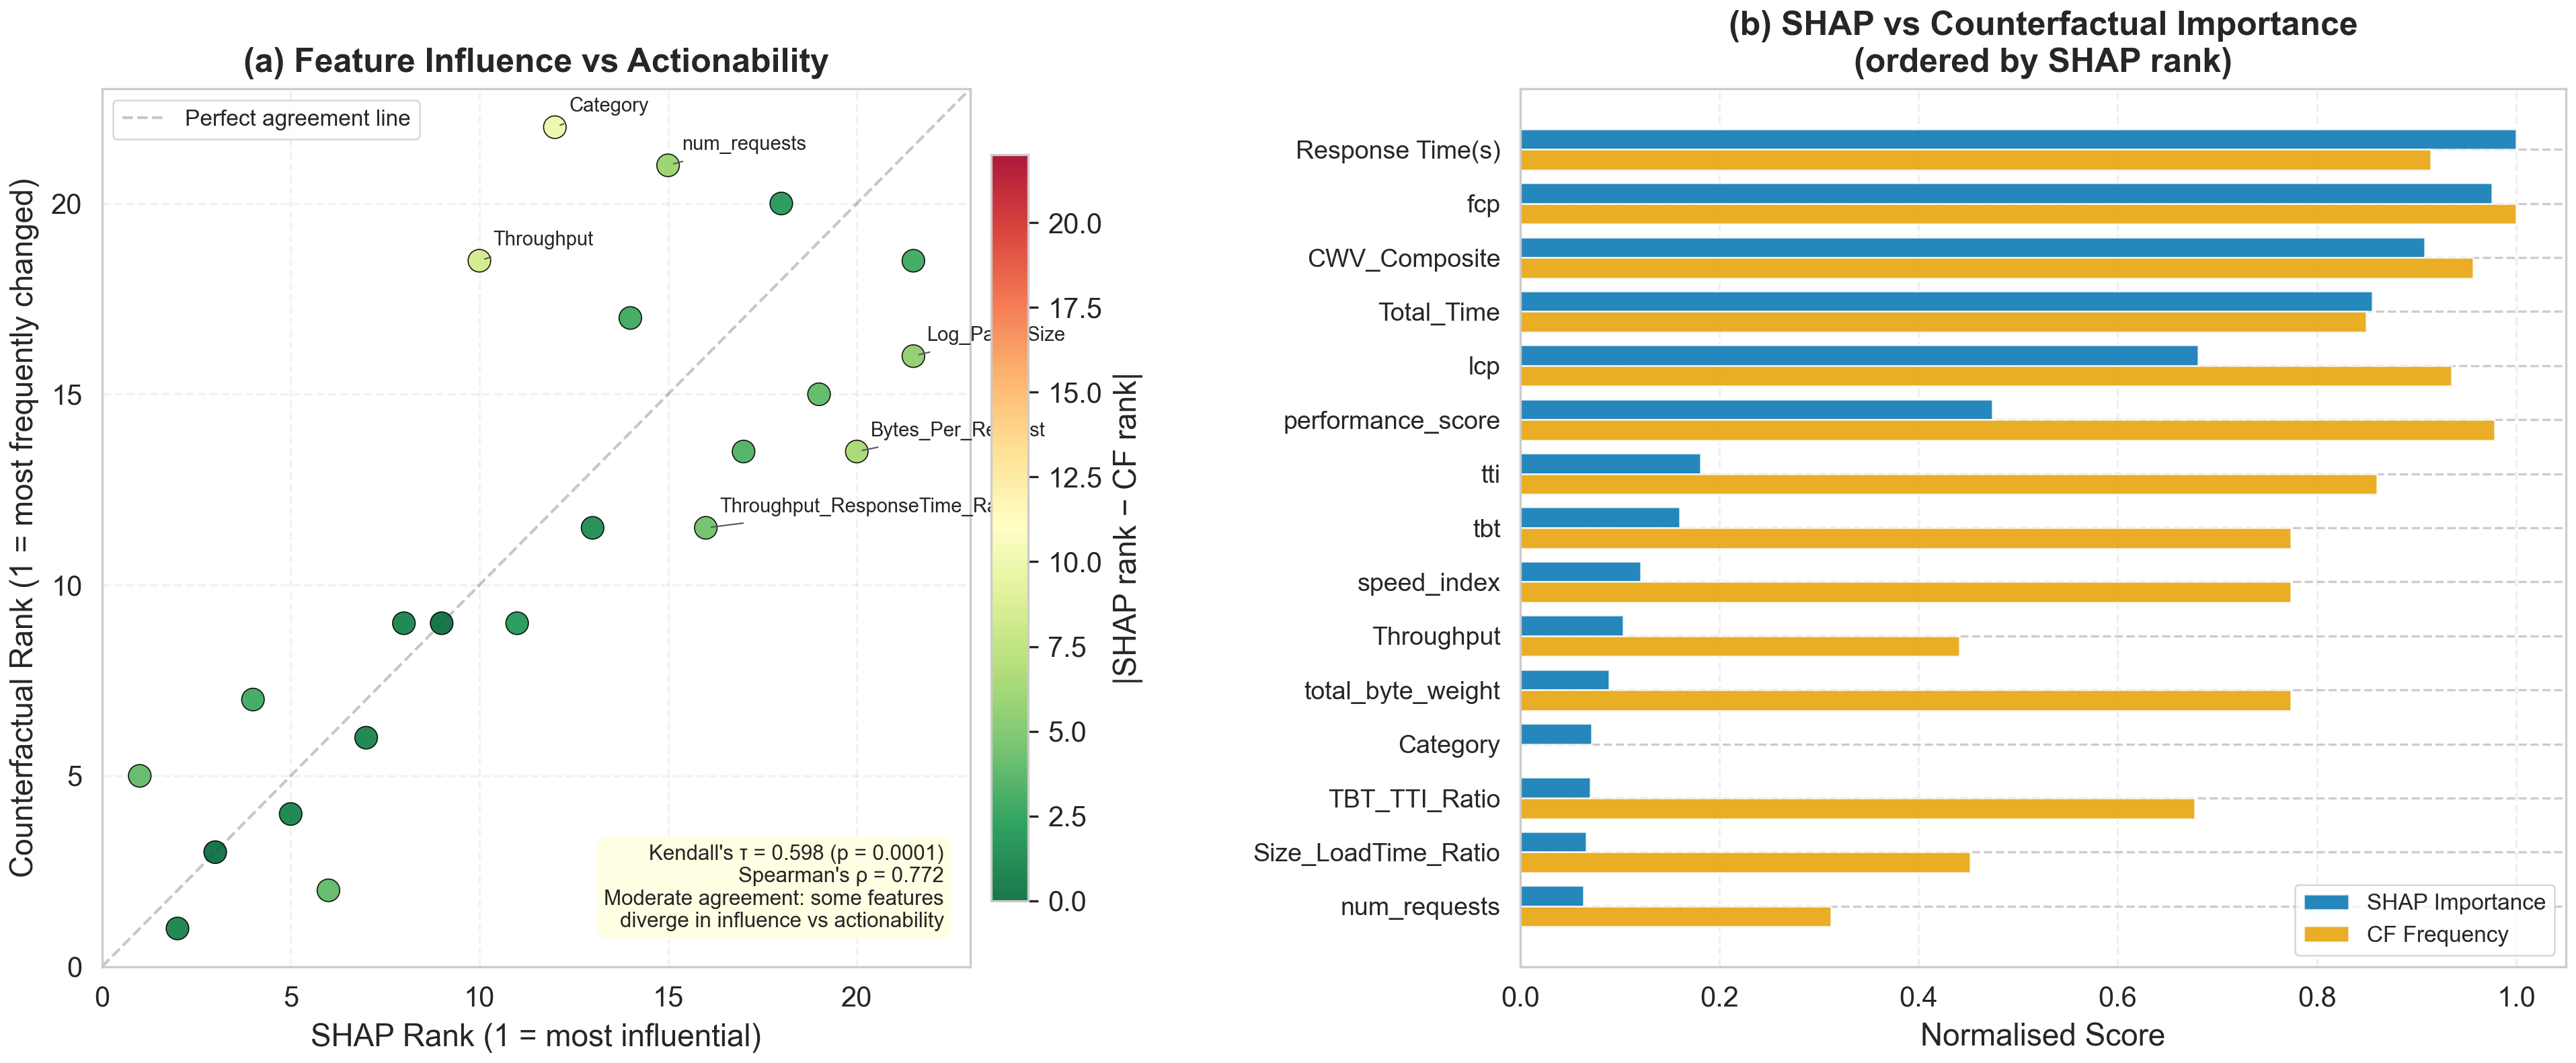
\includegraphics[width=\linewidth]{figures/fig4_shap_vs_counterfactual.png}
    \caption{Feature influence vs.\ feature actionability. (a)~Rank scatter plot: SHAP rank on the $x$-axis, counterfactual frequency rank on the $y$-axis ($\tau = 0.598$, $\rho = 0.772$). Dot colour encodes the absolute rank difference. (b)~Side-by-side normalised SHAP vs.\ CF importance showing that composite timing metrics (\textit{tti}, \textit{tbt}, \textit{TBT\_TTI\_Ratio}) are substantially more actionable than their SHAP rank implies, while Category has high SHAP influence but near-zero actionability.}
    \label{fig:shap_vs_cf}
\end{figure}

\subsection{Real-World Experimental Validation}

Table~\ref{tab:realworld} summarizes the controlled deployment experiment. The model correctly predicted slow for the baseline and fast for the optimized page. The external PageSpeed API independently confirmed both classifications. All prescription targets were met or exceeded, with an average metric improvement of 94.5\% and domain compliance of 92.9\%. Because the audit is performed by an external API entirely separate from the internal model, this experiment directly rules out the circular validation that affects most prior work in this domain.

\begin{table}[htb]
\caption{Real-World Validation Results}\label{tab:realworld}
\centering
\begin{tabular}{lccc}
\toprule
Metric & Baseline & Optimized & Change \\
\midrule
PageSpeed Score & 55 / 100 & 100 / 100 & +81.8\% \\
FCP & 11,167 ms & 854 ms & $-$92.4\% \\
LCP & 31,616 ms & 854 ms & $-$97.3\% \\
TTI & 31,616 ms & 878 ms & $-$97.2\% \\
TBT & 3 ms & 0 ms & $-$100.0\% \\
Page Size & 6,080 KB & 8.85 KB & $-$99.9\% \\
Model $P(\text{fast})$ & 2.74\% & 99.74\% & +97.0 pp \\
\bottomrule
\end{tabular}
\end{table}

\begin{figure}[htb]
    \centering
    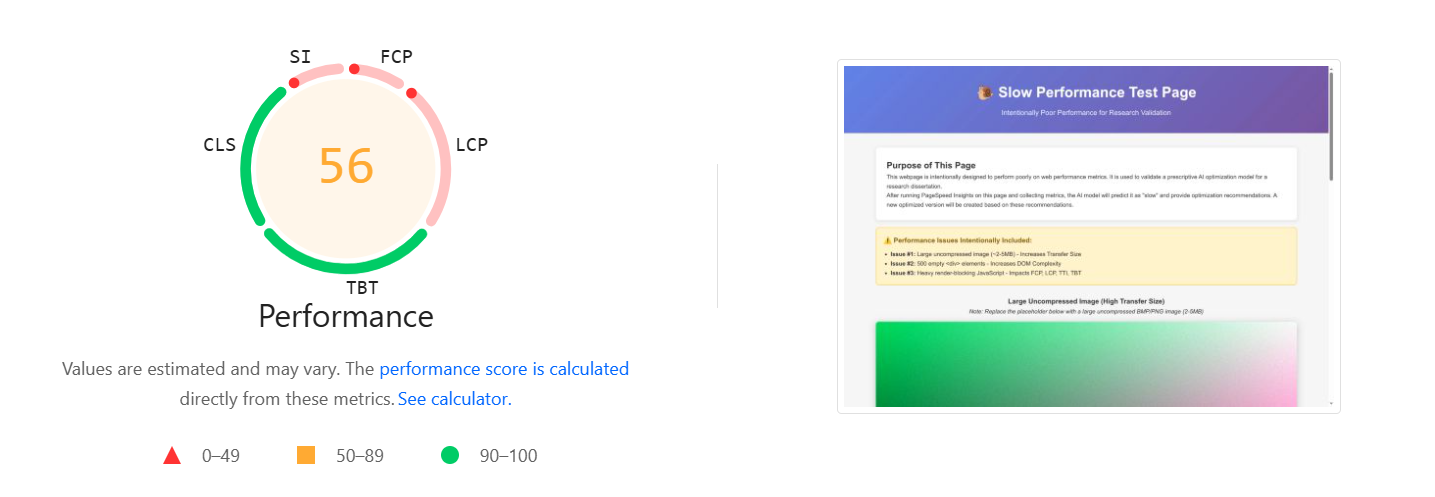
\includegraphics[width=\linewidth]{figures/slowpageperformance.png}\\[6pt]
    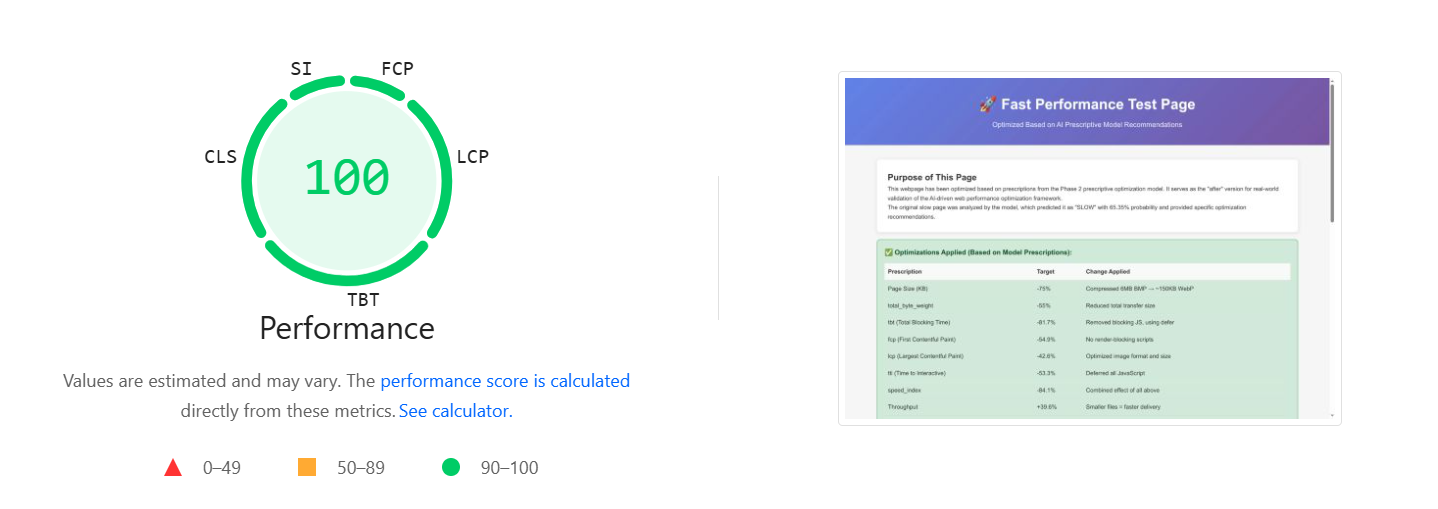
\includegraphics[width=\linewidth]{figures/fastpageperformance.png}
    \caption{Google PageSpeed Insights results for the baseline deployment (score 55, top) and the optimized deployment (score 100, bottom), independently verifying the framework's prescriptions. All prescription targets were met or exceeded, with an average metric improvement of 94.5\% and domain compliance of 92.9\%.}
    \label{fig:pagespeed_screenshots}
\end{figure}

% ====================================================================
%  SECTION 5 - DISCUSSION
% ====================================================================
\section{Discussion}

\textbf{Predictive rigor:} Wrapping the scaler inside cross-validation folds eliminates a subtle but common source of data leakage that inflates reported accuracy in many published studies~\cite{xin2023}. The near-zero test-to-CV gap confirms the model generalizes well to unseen data. The dominance of Response Time, FCP, LCP, and CWV\_Composite across both SHAP and consensus rankings confirms the industry's shift toward perceived performance metrics~\cite{mathur2024,sehwag2024}.

\textbf{Influence vs.\ actionability:} The SHAP-to-counterfactual analysis exposes a distinction that is easy to miss when relying on a single explanation method. Features that strongly influence predictions are not always the features most readily changed to improve a classification outcome~\cite{goldwasser2024,ali2023}. TTI, TBT, and TBT\_TTI\_Ratio have high counterfactual frequency but low SHAP rank, making them effective remediation levers that a SHAP-only practitioner might overlook. Category carries substantial SHAP weight but never appears in counterfactuals, correctly reflecting that site category is a structural covariate and not an optimization target.

\textbf{Category-specific strategies:} Nine of 22 features differ significantly across website categories, meaning that a blanket optimization recipe applied uniformly across news sites, e-commerce portals, and sports platforms will be suboptimal for each. Category-aware prescriptive models are a natural next step.

\textbf{Practical implications:} For practitioners, the framework offers automated decision support by replacing manual waterfall chart audits with a prioritized list of specific changes~\cite{vanriet2023}. The predictive component can also serve as a quality gate in CI/CD pipelines, estimating the performance class of a build before production~\cite{dakic2025}. The XAI layer generates quantifiable evidence (SHAP plots, consensus rankings, counterfactual scenarios) that engineers can use when requesting resources for refactoring or infrastructure investment~\cite{hassija2024}.

\textbf{Limitations:} The primary dataset of 885 pages may not represent all web architectures such as single-page applications and WebGL-heavy sites. The prescriptive engine operates at the feature level rather than the code level, leaving a last-mile gap between recommending a 60\% LCP reduction and generating the specific configuration to achieve it. Mean counterfactual sparsity (13.2 feature changes) is relatively high; incorporating causal discovery to restrict modifications to causally upstream features could improve this. Reliance on the Google PageSpeed Insights API introduces a dependency on external rate limits and evolving scoring algorithms.

% ====================================================================
%  SECTION 6 - CONCLUSION
% ====================================================================
\section{Conclusion}

This paper presented a unified pipeline connecting web performance prediction, prescription, and explanation within a single empirically validated system. An XGBoost classifier inside a leak-proof scikit-learn Pipeline achieves 90.60\% test accuracy, confirmed by three formal statistical tests. The learned representations transfer to 8,000 independently labelled HTTP Archive URLs at 97.54\%, providing strong evidence of cross-dataset generalizability. A Differential Evolution engine with direction-aware constraints achieves 100\% batch prescription success. The explainability layer contributes a fidelity-weighted consensus of SHAP, LIME, and Permutation Importance; quantified LIME stability (Jaccard = 0.876); category-stratified significance testing across 22 features; and counterfactual analysis revealing that timing features such as TTI and TBT are high-leverage remediation targets despite low SHAP importance. A controlled real-world experiment, audited independently by the Google PageSpeed API, reduces LCP by 97.3\% and raises the PageSpeed score from 55 to 100, ruling out circular validation.

Future directions include automated code-level refactoring using large language models, multi-objective optimization balancing performance and energy efficiency for green web engineering, longitudinal monitoring for continuous performance assurance, causal counterfactuals restricting modifications to causally upstream features, and scaling training to the full HTTP Archive for broader generalizability evidence.

% ====================================================================
%  BIBLIOGRAPHY
% ====================================================================
\begin{thebibliography}{29}

\bibitem{ghattas2025}
Ghattas, M., Mora, A.M., Odeh, S.: A Novel Approach for Evaluating Web Page Performance Based on Machine Learning Algorithms and Optimization Algorithms. AI \textbf{6}(2), 19 (2025). \url{doi:10.3390/ai6020019}

\bibitem{sehwag2024}
Sehwag, A., Mishra, A.P., Kargeti, D., Pahadia, D., Mangal, G.: Applying Predictive Prefetching Using Deep Learning and NLP to Shorten Web Page Loading Times. Int.\ J.\ Multidiscip.\ Res.\ (IJFMR) \textbf{6}(2) (2024). \url{doi:10.36948/ijfmr.2024.v06i02.15447}

\bibitem{mathur2024}
Mathur, S., Hasan, Y., Bhargava, D., Bhattacharjee, S., Rana, A.: Artificial Intelligence Based Predictive Analytics for Website Performance Optimization. In: Proc.\ 7th Int.\ Conf.\ Contemporary Computing and Informatics, pp.\ 795--800 (2024)

\bibitem{kaushik2024}
Kaushik, N., Kumar, H., Raj, V.: Micro Frontend Based Performance Improvement and Prediction for Microservices Using Machine Learning. J.\ Grid Comput.\ \textbf{22} (2024). \url{doi:10.1007/s10723-024-09760-8}

\bibitem{xin2023}
Xin, R., Liu, H., Chen, P., Zhao, Z.: Robust and accurate performance anomaly detection and prediction for cloud applications: a novel ensemble learning-based framework. J.\ Cloud Comput.\ \textbf{12} (2023). \url{doi:10.1186/s13677-022-00383-6}

\bibitem{dakic2025}
Daki\'{c}, V., Djambi\'{c}, G., Slovinac, J., Red\v{z}epagi\'{c}, J.: Optimizing Kubernetes Scheduling for Web Applications Using Machine Learning. Electronics \textbf{14}(5), 863 (2025). \url{doi:10.3390/electronics14050863}

\bibitem{huang2023}
Huang, D., Costero, L., Pahlevan, A., Zapater, M., Alonso, D.: Cloud Prophet: A Machine Learning-Based Performance Prediction for Public Clouds. IEEE Trans.\ Sustain.\ Comput.\ (2023). \url{doi:10.1109/TSUSC.2023.3236543}

\bibitem{vanriet2023}
van Riet, J., Malavolta, I., Ghaleb, T.A.: Optimize along the way: An industrial case study on web performance. J.\ Syst.\ Softw.\ \textbf{198}, 111593 (2023). \url{doi:10.1016/j.jss.2022.111593}

\bibitem{notz2024}
Notz, P.M., Pibernik, R.: Explainable subgradient tree boosting for prescriptive analytics in operations management. Eur.\ J.\ Oper.\ Res.\ \textbf{312}(3), 1119--1133 (2024). \url{doi:10.1016/j.ejor.2023.08.037}

\bibitem{asha2025}
Asha, M.M., Ramya, G.: Predator crow search optimization with explainable AI for cardiac vascular disease classification. Sci.\ Rep.\ \textbf{15} (2025). \url{doi:10.1038/s41598-025-96003-9}

\bibitem{goscien2025}
Go\'{s}cie\'{n}, R.: Explainable artificial intelligence-based framework for efficient content placement in elastic optical networks. Expert Syst.\ Appl.\ \textbf{262}, 125541 (2025). \url{doi:10.1016/j.eswa.2025.125541}

\bibitem{surianarayanan2023}
Surianarayanan, C., Lawrence, J.J., Chelliah, P.R., Prakash, E., Hewage, C.: A Survey on Optimization Techniques for Edge Artificial Intelligence (AI). Sensors \textbf{23}(3), 1279 (2023). \url{doi:10.3390/s23031279}

\bibitem{liu2023}
Liu, B., Vu-Bac, N., Zhuang, X., Lu, W., Fu, X., Rabczuk, T.: AI-DeMat: A web-based expert system platform for computationally expensive models in materials design. Adv.\ Eng.\ Softw.\ \textbf{176}, 103361 (2023). \url{doi:10.1016/j.advengsoft.2022.103361}

\bibitem{yang2025}
Yang, X., et al.: Machine learning-driven clinical decision support for low bone mineral density: A web-based prediction model with explainable AI integration. Bone \textbf{200}, 117592 (2025). \url{doi:10.1016/j.bone.2025.117592}

\bibitem{salih2024}
Salih, A.M., et al.: A Perspective on Explainable Artificial Intelligence Methods: SHAP and LIME. Adv.\ Intell.\ Syst.\ (2024). \url{doi:10.1002/aisy.202400304}

\bibitem{hassija2024}
Hassija, V., et al.: Interpreting Black-Box Models: A Review on Explainable Artificial Intelligence. Cogn.\ Comput.\ \textbf{16}, 45--74 (2024). \url{doi:10.1007/s12559-023-10179-8}

\bibitem{ortigossa2024}
Ortigossa, E., Gon\c{c}alves, T., Nonato, L.: EXplainable Artificial Intelligence (XAI) -- From Theory to Methods and Applications. IEEE Access \textbf{12}, 80799--80846 (2024). \url{doi:10.1109/ACCESS.2024.3409843}

\bibitem{goldwasser2024}
Goldwasser, J., Hooker, G.: Provably Stable Feature Rankings with SHAP and LIME. Preprint, arXiv:2401.15800 (2024). \url{doi:10.48550/arXiv.2401.15800}

\bibitem{mersha2024}
Mersha, M., Lam, K.N., Wood, J., AlShami, A., Kalita, J.: Explainable artificial intelligence: A survey of needs, techniques, applications, and future direction. Neurocomputing \textbf{599} (2024). \url{doi:10.1016/j.neucom.2024.128111}

\bibitem{bennetot2024}
Bennetot, A., et al.: A Practical Tutorial on Explainable AI Techniques. ACM Comput.\ Surv.\ \textbf{57} (2024). \url{doi:10.1145/3670685}

\bibitem{ali2023}
Ali, S., et al.: Explainable Artificial Intelligence (XAI): What we know and what is left to attain Trustworthy Artificial Intelligence. Inf.\ Fusion \textbf{99}, 101805 (2023). \url{doi:10.1016/j.inffus.2023.101805}

\bibitem{hosain2024}
Hosain, M., Jim, J., Mridha, M., Kabir, M.: Explainable AI approaches in deep learning: Advancements, applications and challenges. Comput.\ Electr.\ Eng.\ \textbf{117}, 109246 (2024). \url{doi:10.1016/j.compeleceng.2024.109246}

\bibitem{zhou2024}
Sharma, N.A., et al.: Explainable AI Frameworks: Navigating the Present Challenges and Unveiling Innovative Applications. Algorithms \textbf{17}(6), 227 (2024). \url{doi:10.3390/a17060227}

\bibitem{goyal2025}
Goyal, B.: Explainable AI (XAI) for Cloud-Based Enterprise Applications: Building Trust and Transparency in AI-Driven Decisions. J.\ Int.\ Crisis Risk Commun.\ Res.\ \textbf{8}(S9), 63--71 (2025). \url{doi:10.63278/jicrcr.vi.3231}

\bibitem{alam2024}
Alam, K., Kifayat, K., Sampedro, G.A., Karovic, V., Naeem, T.: SXAD: Shapely eXplainable AI-Based Anomaly Detection Using Log Data. IEEE Access \textbf{12}, 95659--95672 (2024). \url{doi:10.1109/ACCESS.2024.3425472}

\bibitem{benleulmi2025}
Benleulmi, M., Gasmi, I., Azizi, N., Dey, N.: Explainable AI and Deep Learning Models for Recommender Systems: State of the Art and Challenges. J.\ Univers.\ Comput.\ Sci.\ \textbf{31}(4), 383--421 (2025). \url{doi:10.3897/jucs.122380}

\bibitem{rahim2025}
Rahim~M, N., Basheer~K.P, M.: A Hybrid Explainability Framework for Recommender Systems Using SHAP with Natural Language Interpretations. Int.\ J.\ Innov.\ Res.\ Sci.\ Stud.\ \textbf{8}(6), 687--703 (2025). \url{doi:10.53894/ijirss.v8i6.9669}

\bibitem{mersha2025}
Mersha, M., et al.: Explainable AI: XAI-guided context-aware data augmentation. Expert Syst.\ Appl.\ \textbf{289}, 128364 (2025). \url{doi:10.1016/j.eswa.2025.128364}

\bibitem{bhardwaj2025}
Bhardwaj, T., Sumangali, K.: An explainable federated blockchain framework with privacy-preserving AI optimization for securing healthcare data. Sci.\ Rep.\ \textbf{15}, 21799 (2025). \url{doi:10.1038/s41598-025-04083-4}

\end{thebibliography}

\end{document}